\documentclass{article}
\usepackage{arxiv}

\usepackage{hyperref}
\usepackage{url}
\usepackage{amsmath}
\usepackage{mathrsfs}
\usepackage{bm}
\usepackage{amsthm}
\usepackage{amssymb}
\usepackage{array}
\usepackage[dvipsnames]{xcolor}
\usepackage{graphicx} 
\usepackage{booktabs} % for professional tables
\usepackage{makecell} 
\usepackage[figuresright]{rotating}
\usepackage{mathtools}
\usepackage{makecell}
\usepackage{enumitem}
\usepackage{subcaption}
\renewcommand\theadfont{\scriptsize}

% load shortex containing useful packages and shorthand notation
\usepackage[numbers]{natbib}
\bibliographystyle{abbrvnat}
\usepackage[utf8]{inputenc} % allow utf-8 input
\usepackage[T1]{fontenc}    % use 8-bit T1 fonts
\usepackage{url}            % simple URL typesetting
\usepackage{booktabs}       % professional-quality tables

% Latin
\usepackage{xspace}
\newcommand{\eg}{\textit{e.g.}\xspace}
\newcommand{\ie}{\textit{i.e.}\xspace}
\newcommand{\cf}{\textit{cf.}\xspace}
\def\wrt{w.r.t.\xspace}

% useful macros
\def\note#1{\textcolor{blue}{\textbf{Note}: #1}\xspace}
\def\code#1{\colorbox{gray!15}{\small \textcolor{Bittersweet}{\texttt{#1}}}}
\def\todo#1{\textcolor{blue}{\textbf{Todo}: #1}\xspace} 
\def\eqnote#1{\intertext{(\raggedleft #1)}}




% additional macros for highlighting
\usepackage{shortex-light} % needs to be loaded after hyperref
\definecolor{mypurple}{rgb}{0.478, 0.369, 1.0}
\definecolor{myblue}{rgb}{0.2, 0.6, 1.0}
\definecolor{mygreen}{rgb}{0.2, 0.667, 0.2}

%%%%%%%%%%%%%%%%%%%%%%%%%%%%%%%%%%%%%%%%%%%%%%%%%%%%%%%%%%%%%%%%%%%%%%%%%%%%%%%%%%%%%%%%%%%%%%%%%%%%%%%%%%%
\newcommand{\BigO}{\mathcal{O}}


%%%%%%%%%%%%%%%%%%%%%%%%%%%%%%%%%%%%%%%%%%%%%%%%%%%%%%%%%%%%%%%%%%%%%%%%%%%%%%%%%%%%%%%%%%%%%%%%%%%%%%%%%%%
% Fill out paper:
\begin{document}
\title{LLM Notes}

\date{\today}                       
\maketitle
\tableofcontents
\clearpage


\section{Attention}
\subsection{Self Attention}
Given input $\bX \in \reals^{T \times D}$ where $T$ is the sequence length and $D$ is the embedding dimension, we have
\[
\bQ = \bW_Q \bX \in \reals^{T \times d_k} \quad \bK= \bW_K \bX \in \reals^{T \times d_k} \quad \bV = \bW_V \bX \in \reals^{T \times d_v}
\]
\[
\text{Attn}(\bQ, \bK, \bV) = \text{softmax} \left(\frac{\bQ \bK^\top}{\sqrt{d_k}} \right) \bV
\]

\begin{figure}[h]
\centering
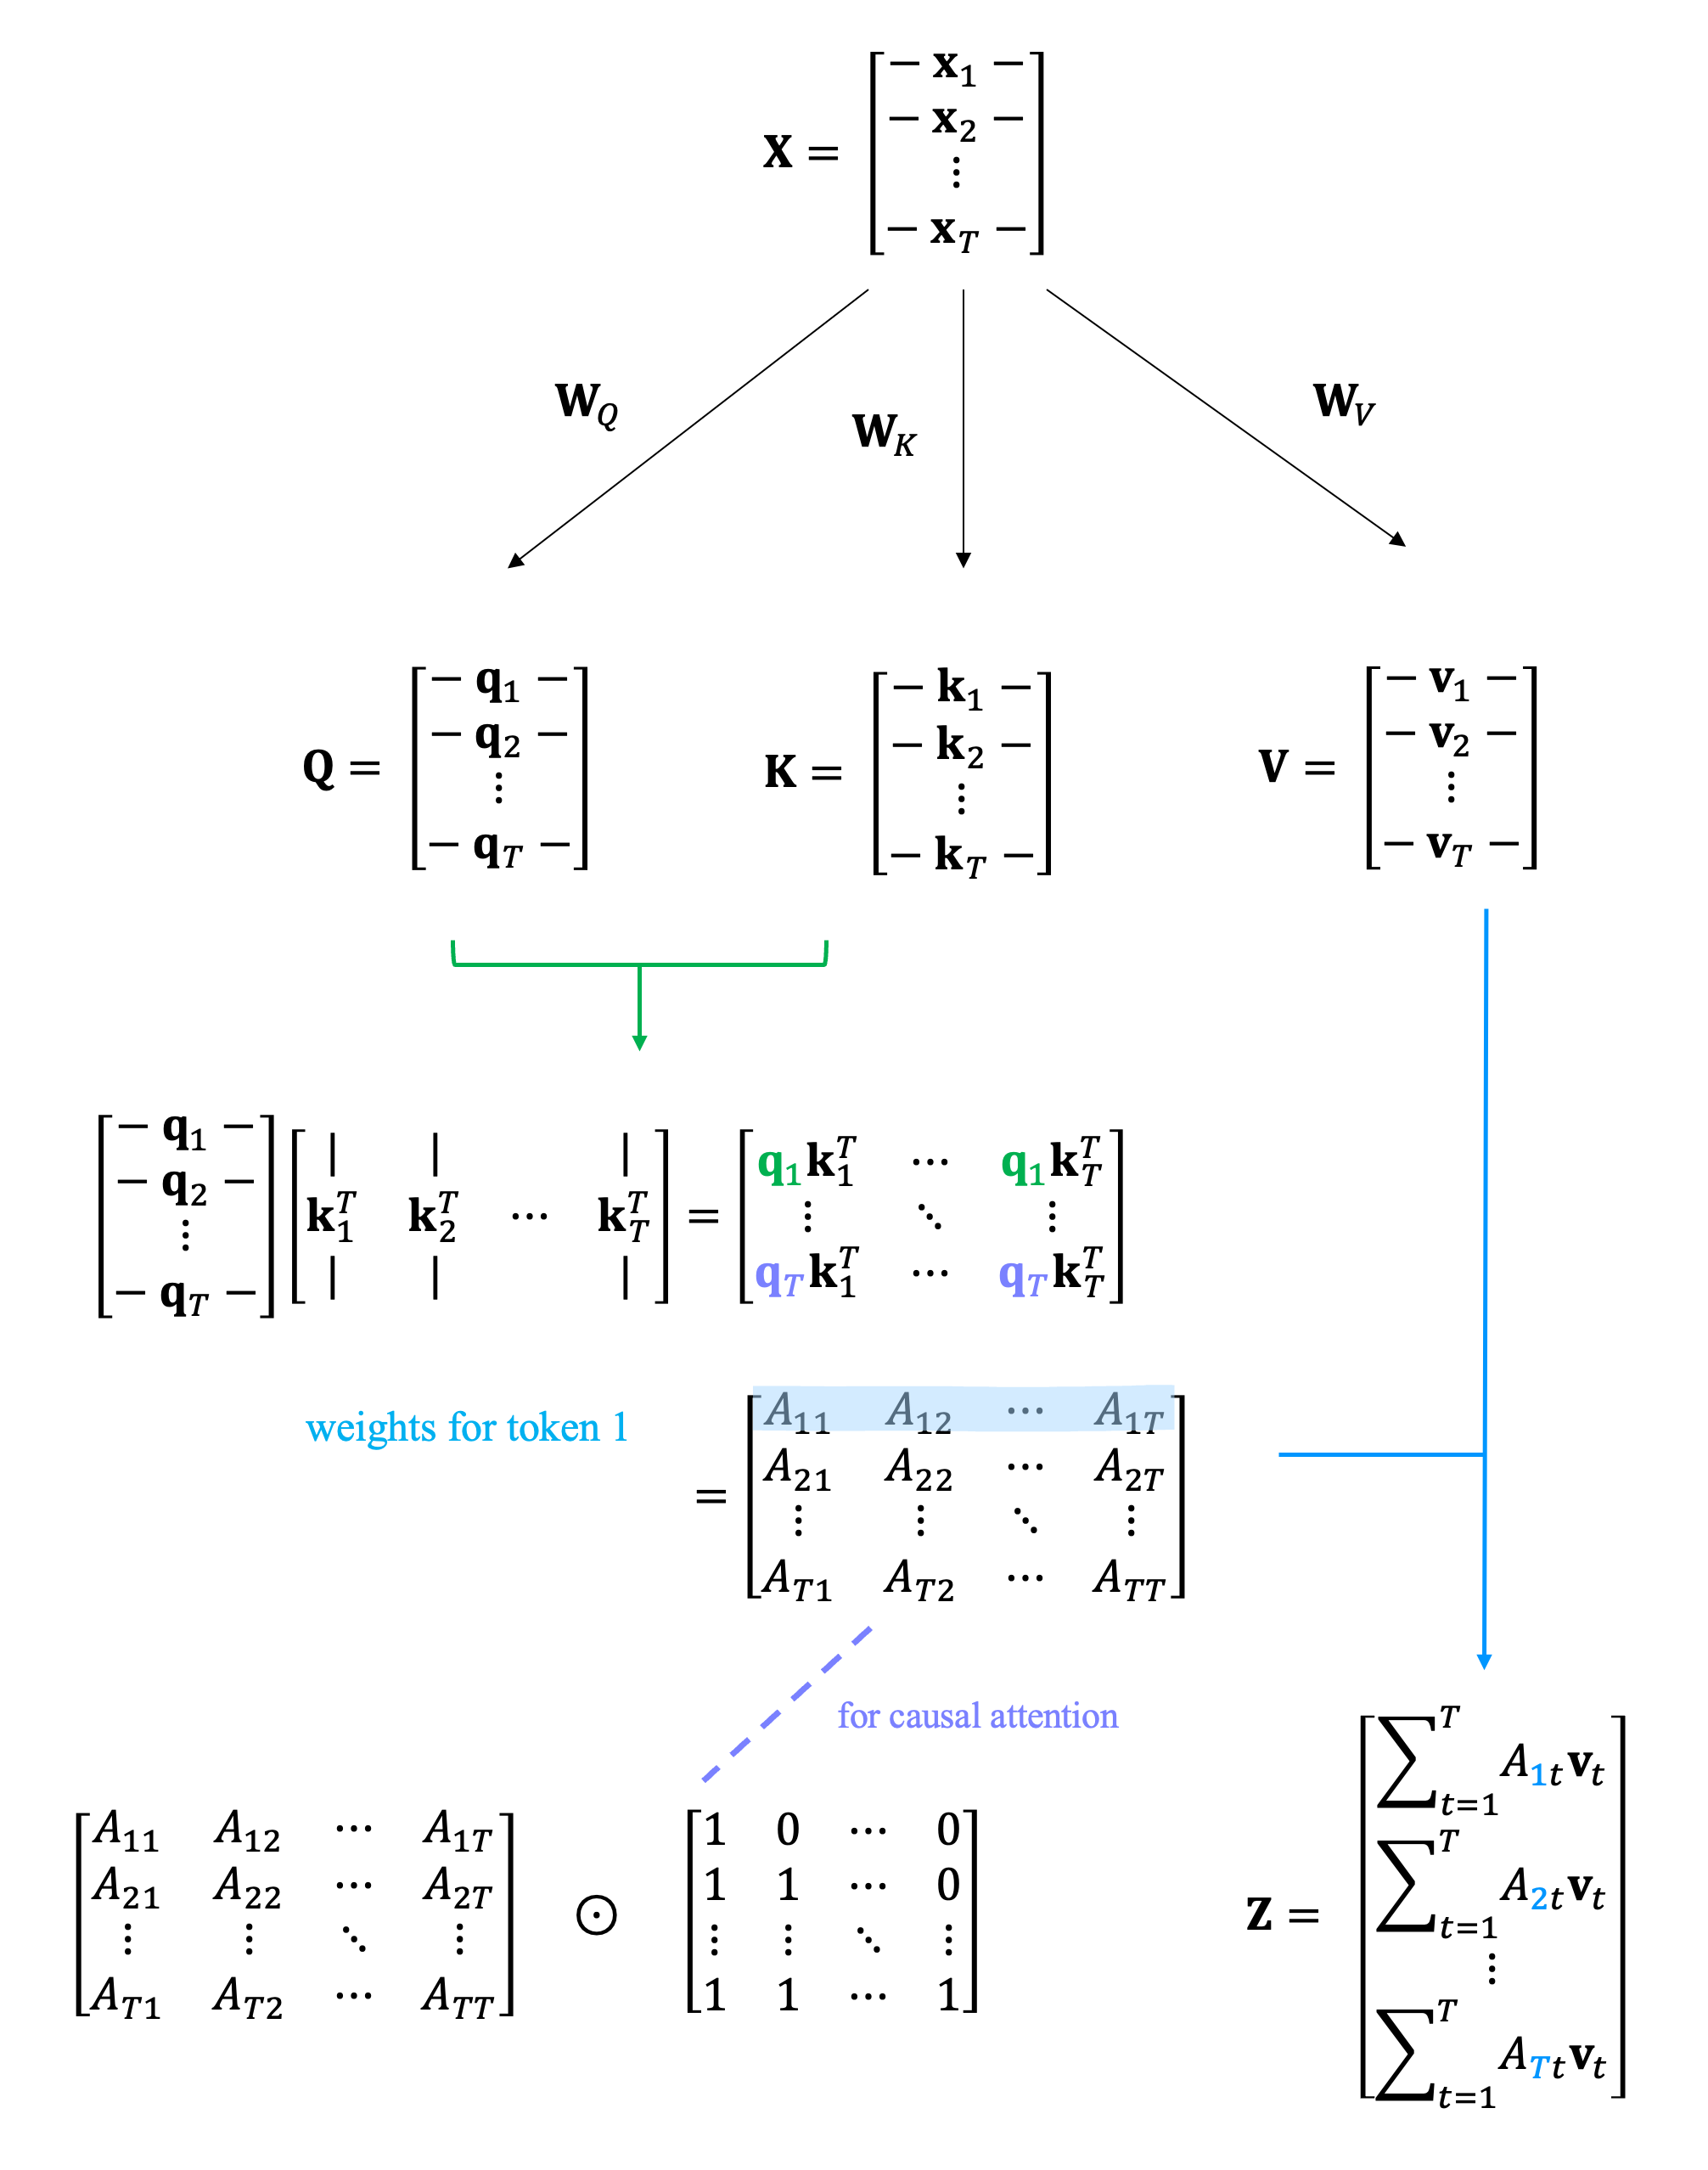
\includegraphics[scale=0.35]{imgs/self-attention.png}
\end{figure}

\clearpage
\subsection{Multi-Head Attention}
In multi-head attention, input $\bX$ is first passed through $H$ self-attention layer in parallel.
Then, the output from each head is concatenated together and fused by a linear projection
\[
\left[\textcolor{myblue}{\bZ^{(1)}}, \bZ^{(2)}, \ldots,  \bZ^{(H)}\right] \bW^O &= 
\begin{bmatrix}
\textcolor{myblue}{\bz_1^{(1)}} &  \bz_1^{(2)} & \ldots & \bz_1^{(H)} \\[0.8em]
\textcolor{myblue}{\bz_2^{(1)}} & \bz_2^{(2)} & \ldots & \bz_2^{(H)} \\[0.8em]
\vdots & \vdots & \ldots & \vdots \\[0.8em]
\textcolor{myblue}{\bz_T^{(1)}} & \bz_T^{(2)} & \ldots & \bz_T^{(H)}
\end{bmatrix}\bW^O
\] 

\begin{figure}[h]
\centering
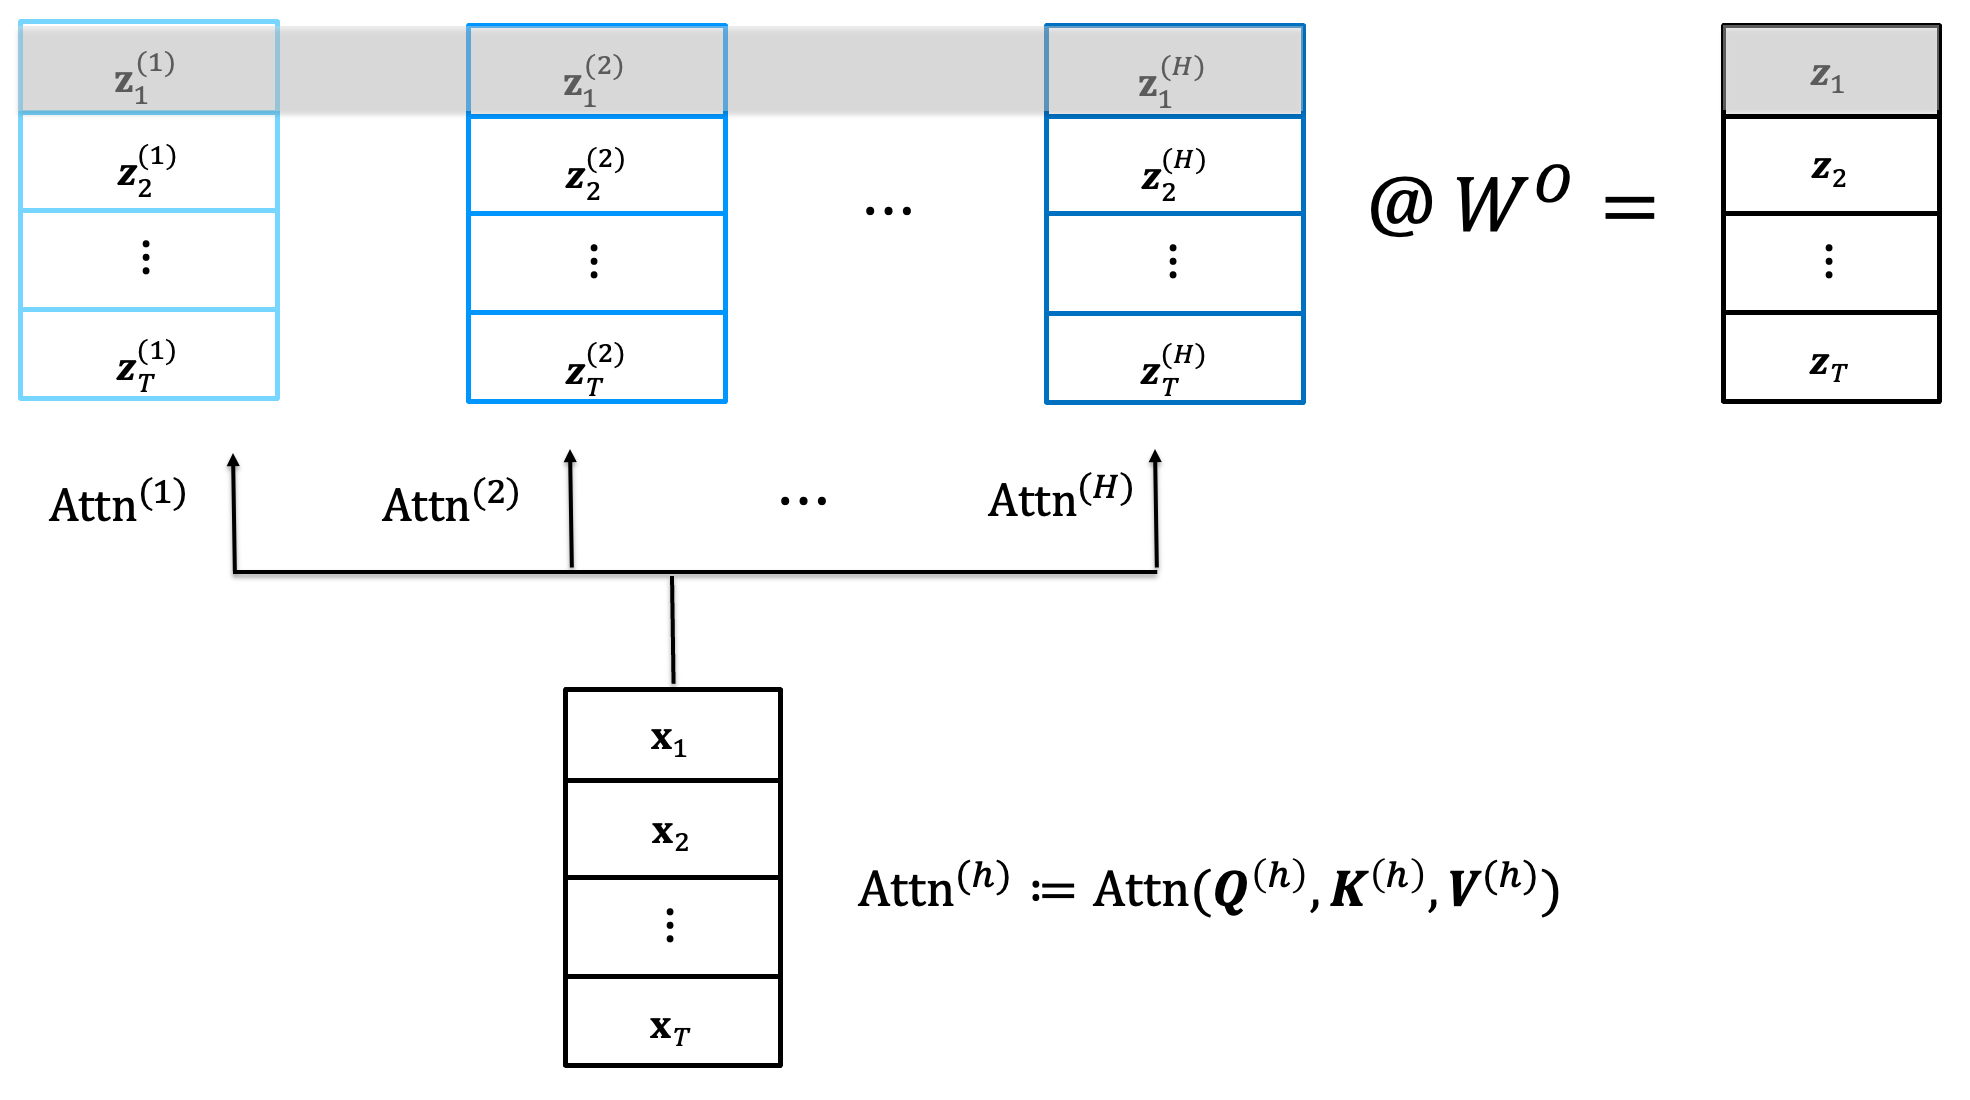
\includegraphics[scale=0.4]{imgs/multi-head.png}
\end{figure}

\clearpage
\subsection{KV-Cache}
During inference we still use causal masking because this is how the model being trained.
Let's look at a simple case where we only give the model a start token <s> and asks it to generate stuff:
\begin{figure}[!h]
\centering
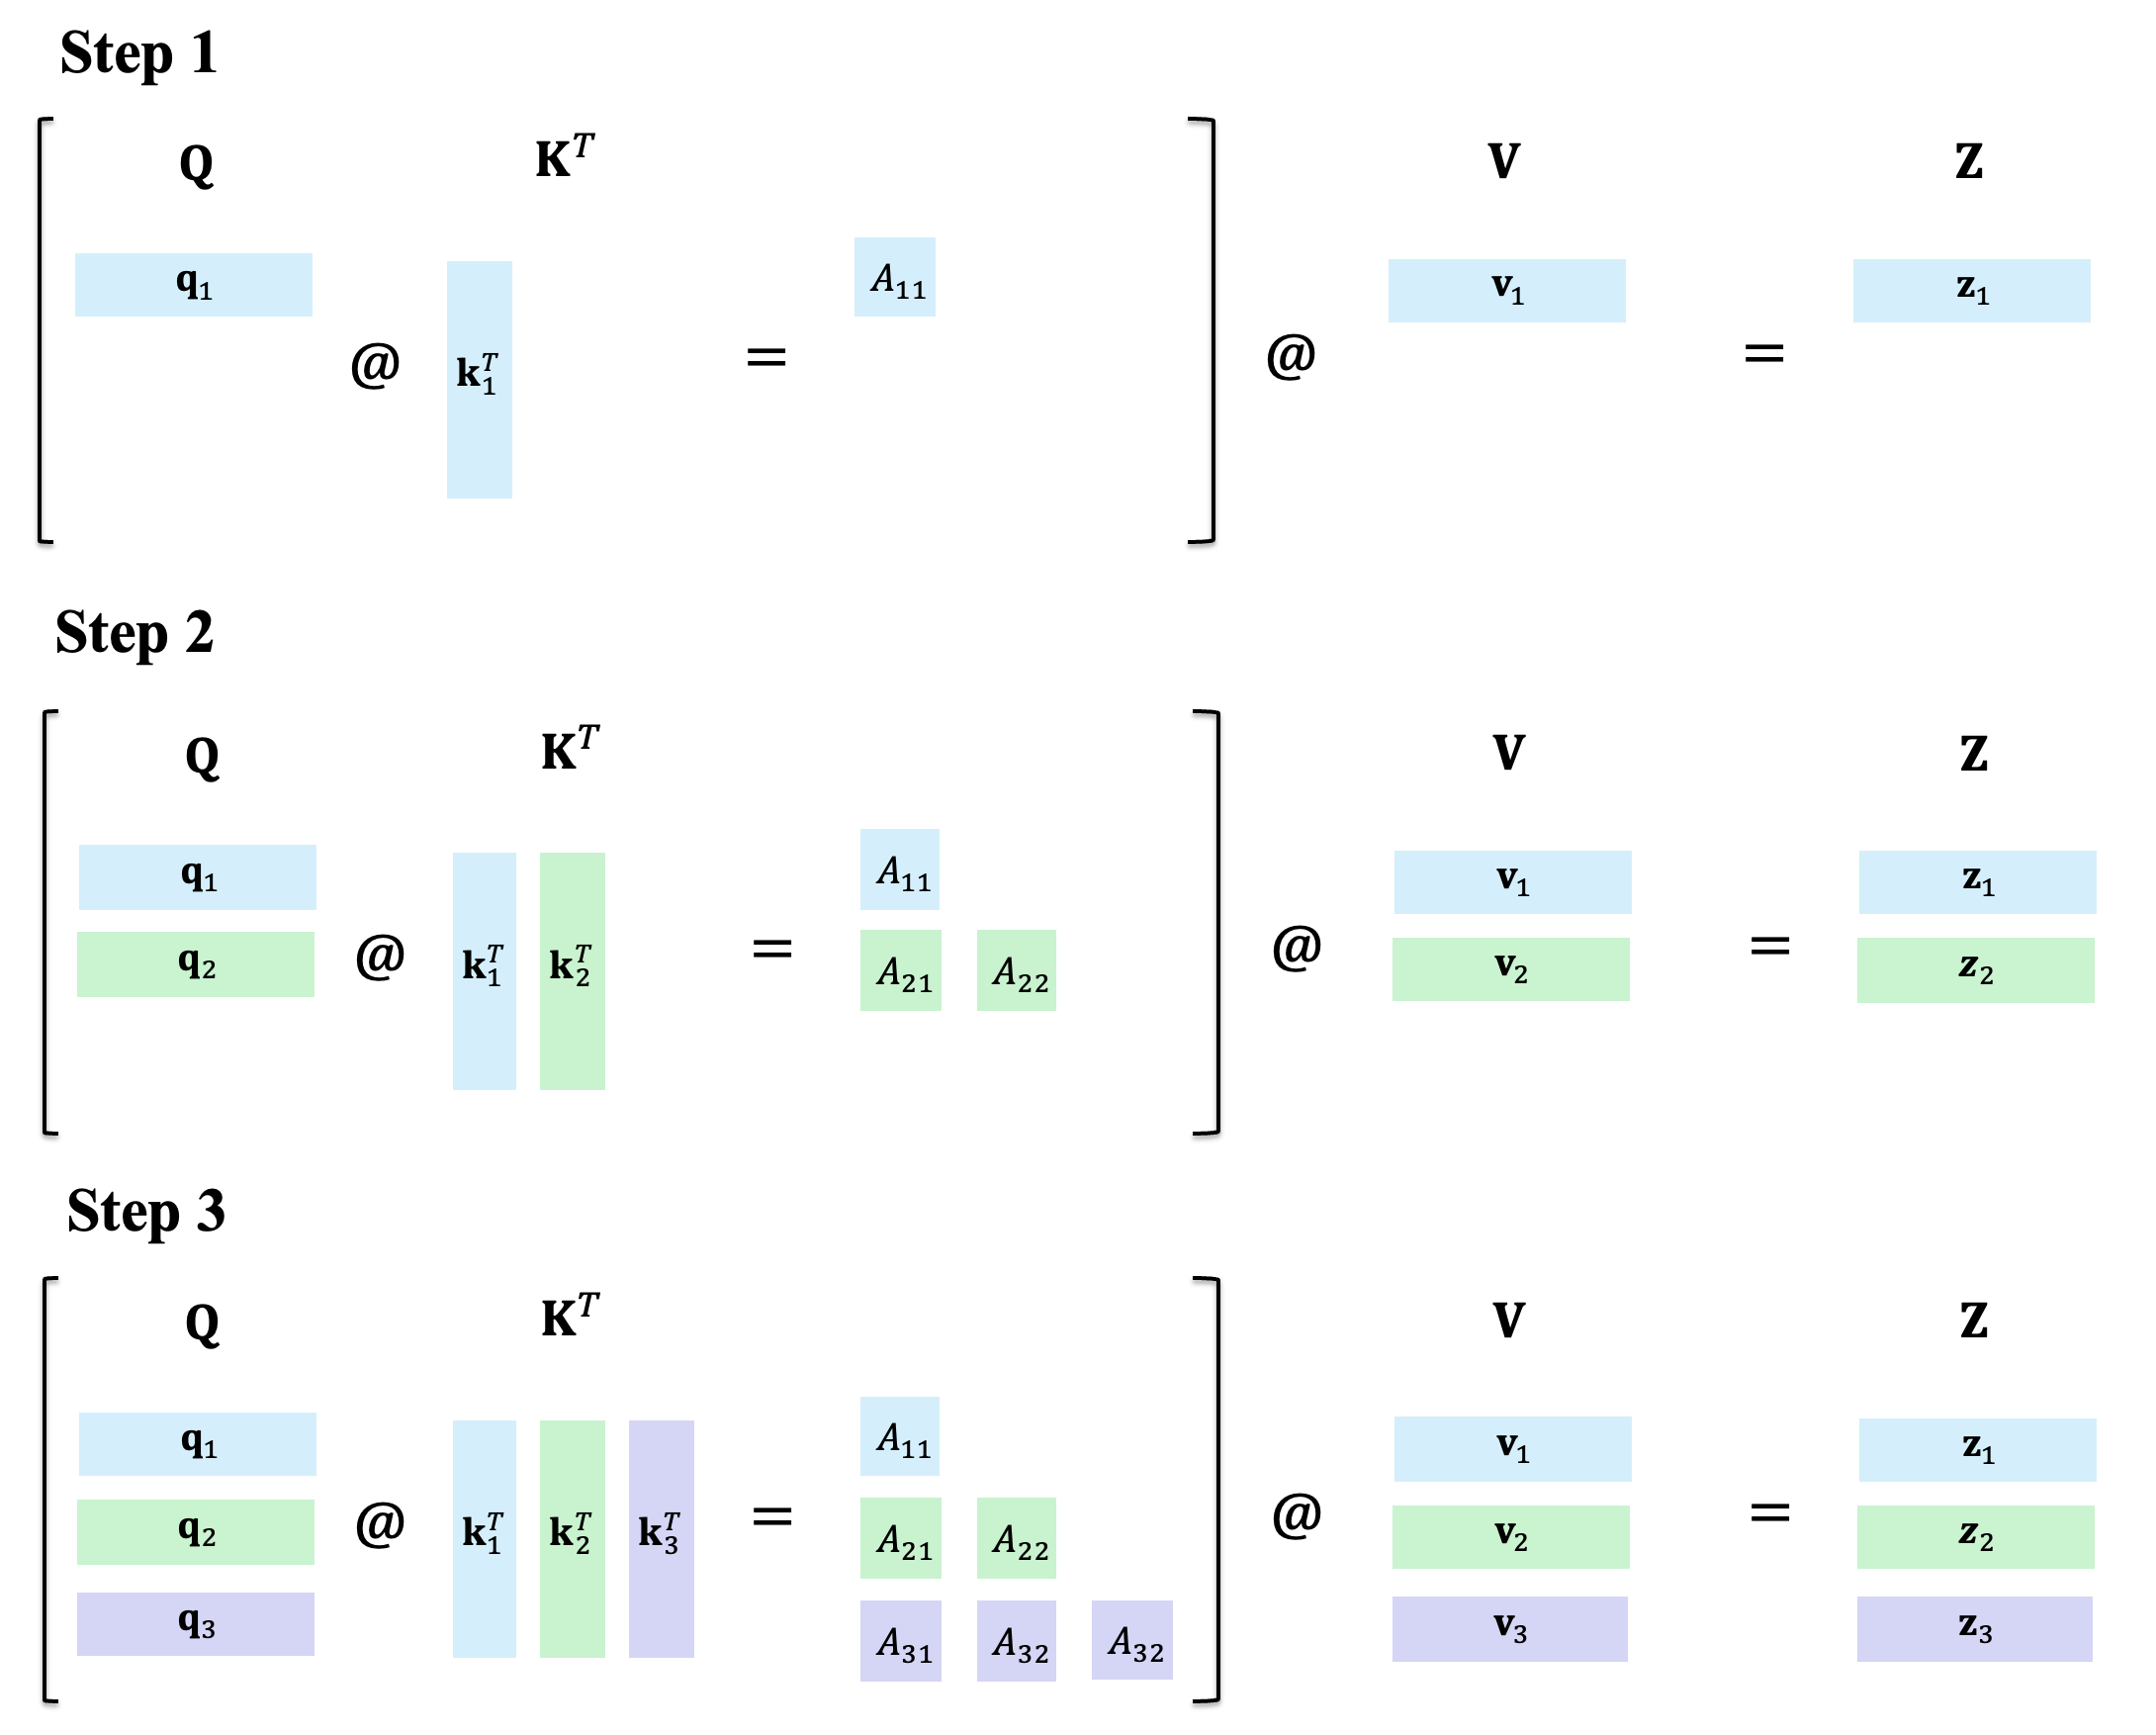
\includegraphics[scale=0.28]{imgs/no-cache.png}
\end{figure}

KV-cache is built on this two observations:
\begin{itemize}
	\item At each time step $t$, due to causal masking $\bk_{<t}$ and $\bv_{<t}$ will remain the same
	\item To predict <$\text{token}_{t+1}$> we only need embedding of <$\text{token}_{t}$>.
\end{itemize}
Therefore, we can make prediction efficiently by drop redundant and unnecessary computation
\begin{figure}[!h]
\centering
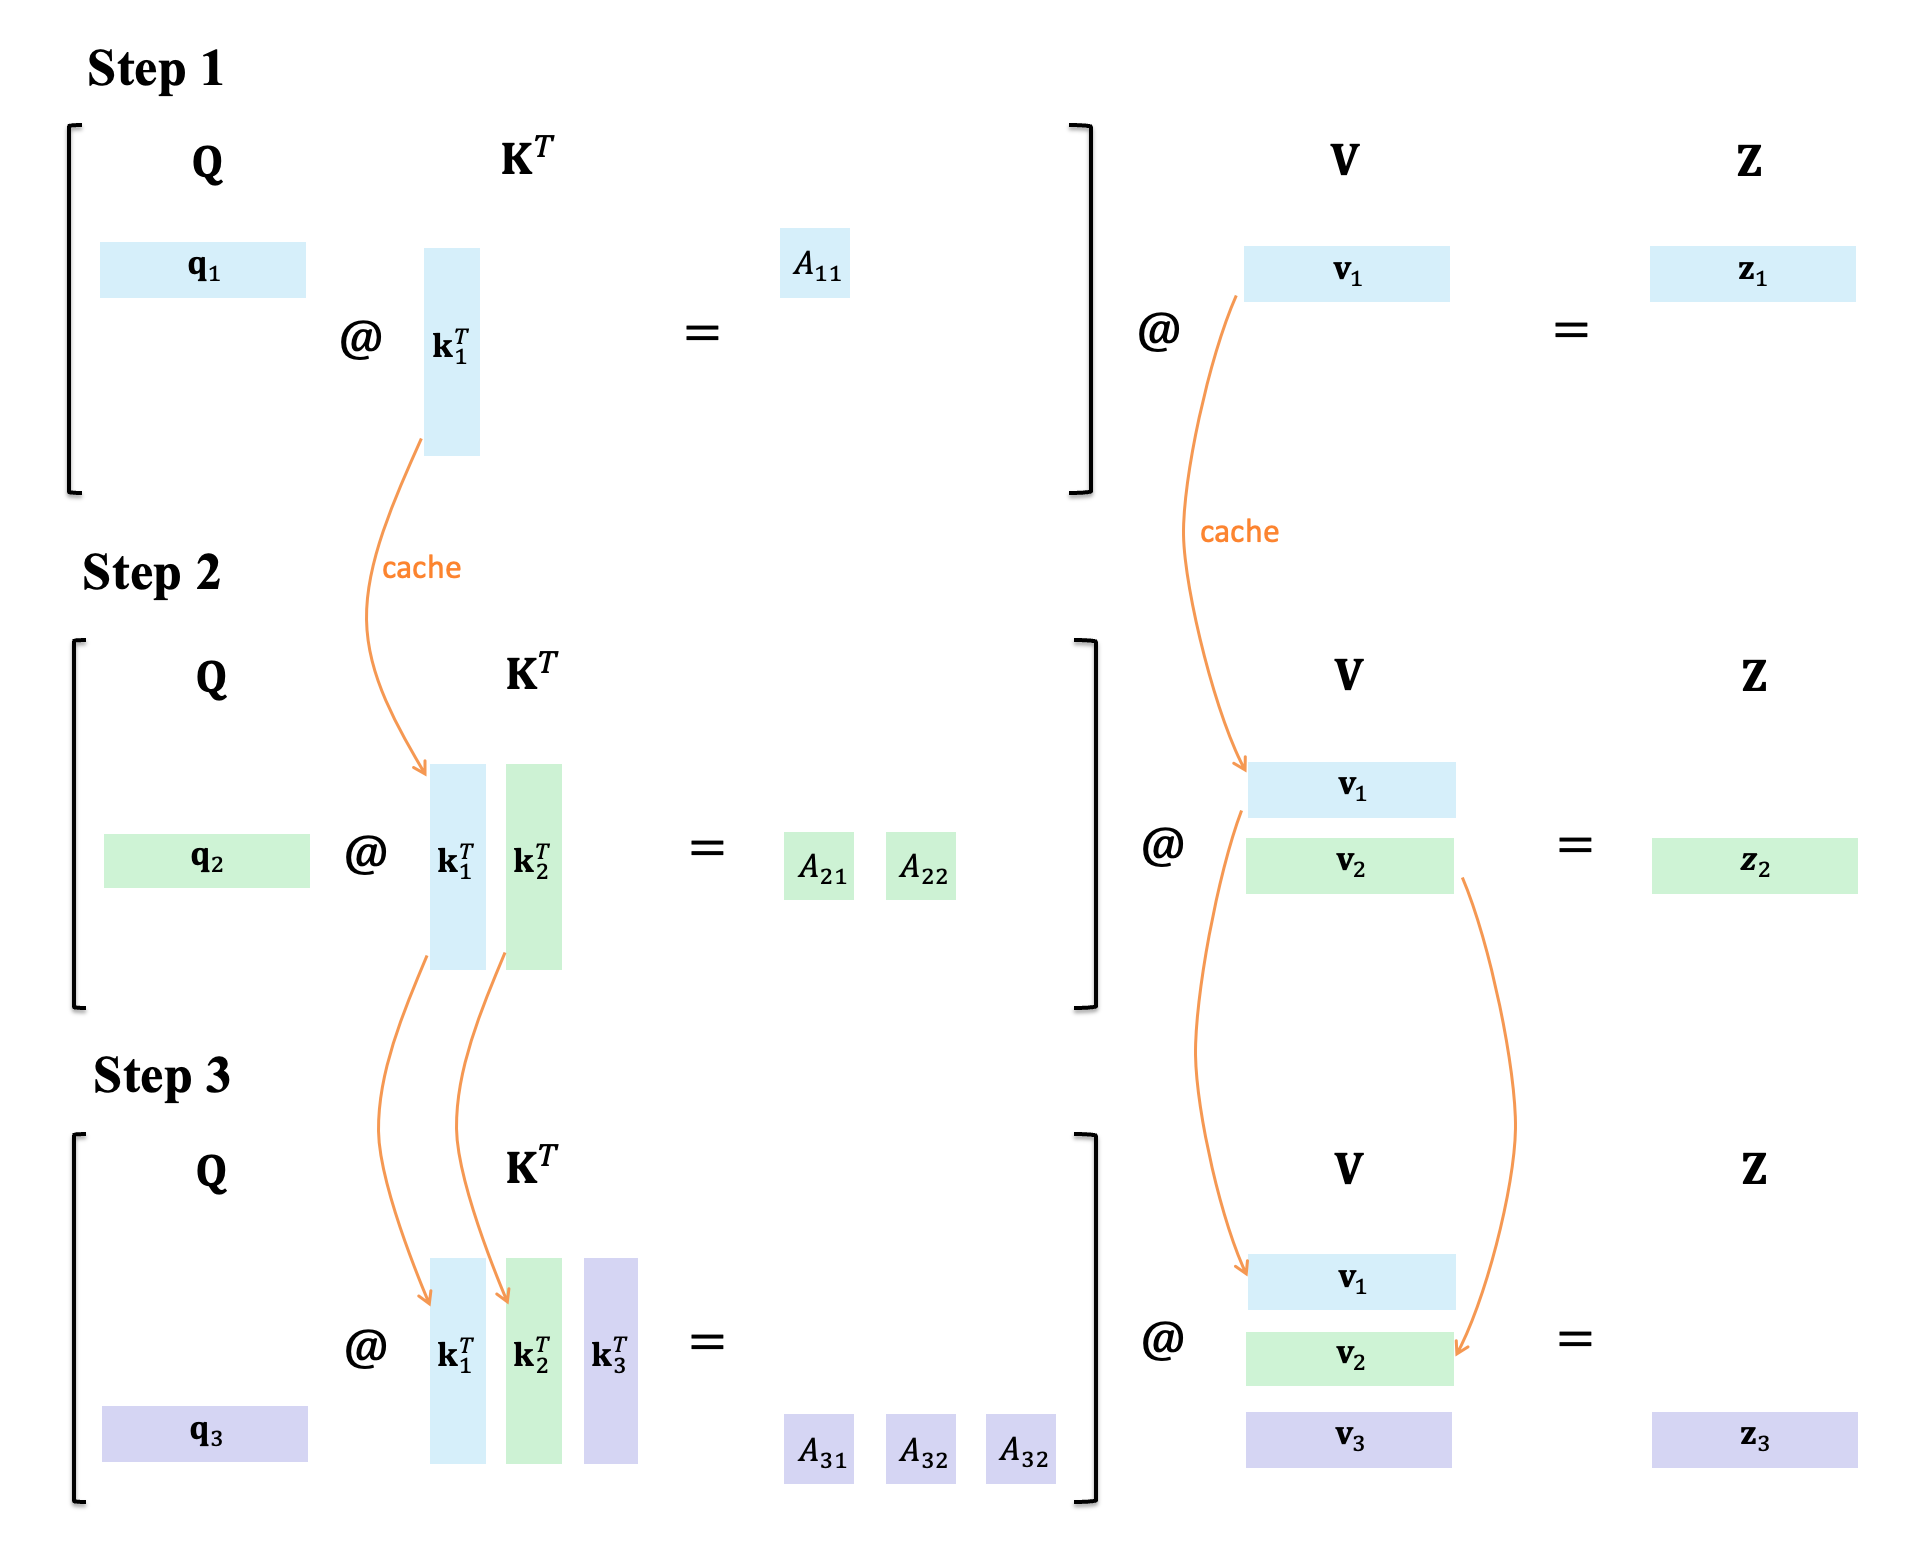
\includegraphics[scale=0.28]{imgs/cache.png}
\end{figure}


\subsection{Multi-Query Attention}
In KV-cache, at time step $t$, the past $t-1$ keys and values are cached, which corresponds to $2 * n_h * (t-1) * h_s$ memory. 
When $t$ gets larger, storing them all on a single GPU will be impossible and the loading will slow things down.

The idea of multi-query attention (MQA) is quite simple. 
In MHA, different heads have different query, key and value projection matrix.
In MQA, the key and value projection matrics will be shared across all heads, only query project matrix will be different:
\[
\begin{array}{ll}
   \text{MHA} & \qquad \text{MQA} \\
  \bQ^{(h)} = \bW_Q^{(h)} \bX & \qquad  \bQ^{(h)} = \bW_Q^{(h)} \bX \\
  \bK^{(h)} = \bW_K^{(h)} \bX & \qquad  \bK^{(h)} = \bW_K \bX \quad \text{(shared across heads)} \\
  \bV^{(h)} = \bW_V^{(h)} \bX & \qquad  \bV^{(h)} = \bW_V \bX \quad \text{(shared across heads)}
\end{array}
\]

This way, we only need to store one set of KV-cache and share it across all heads.
\begin{figure}[!h]
	\centering
	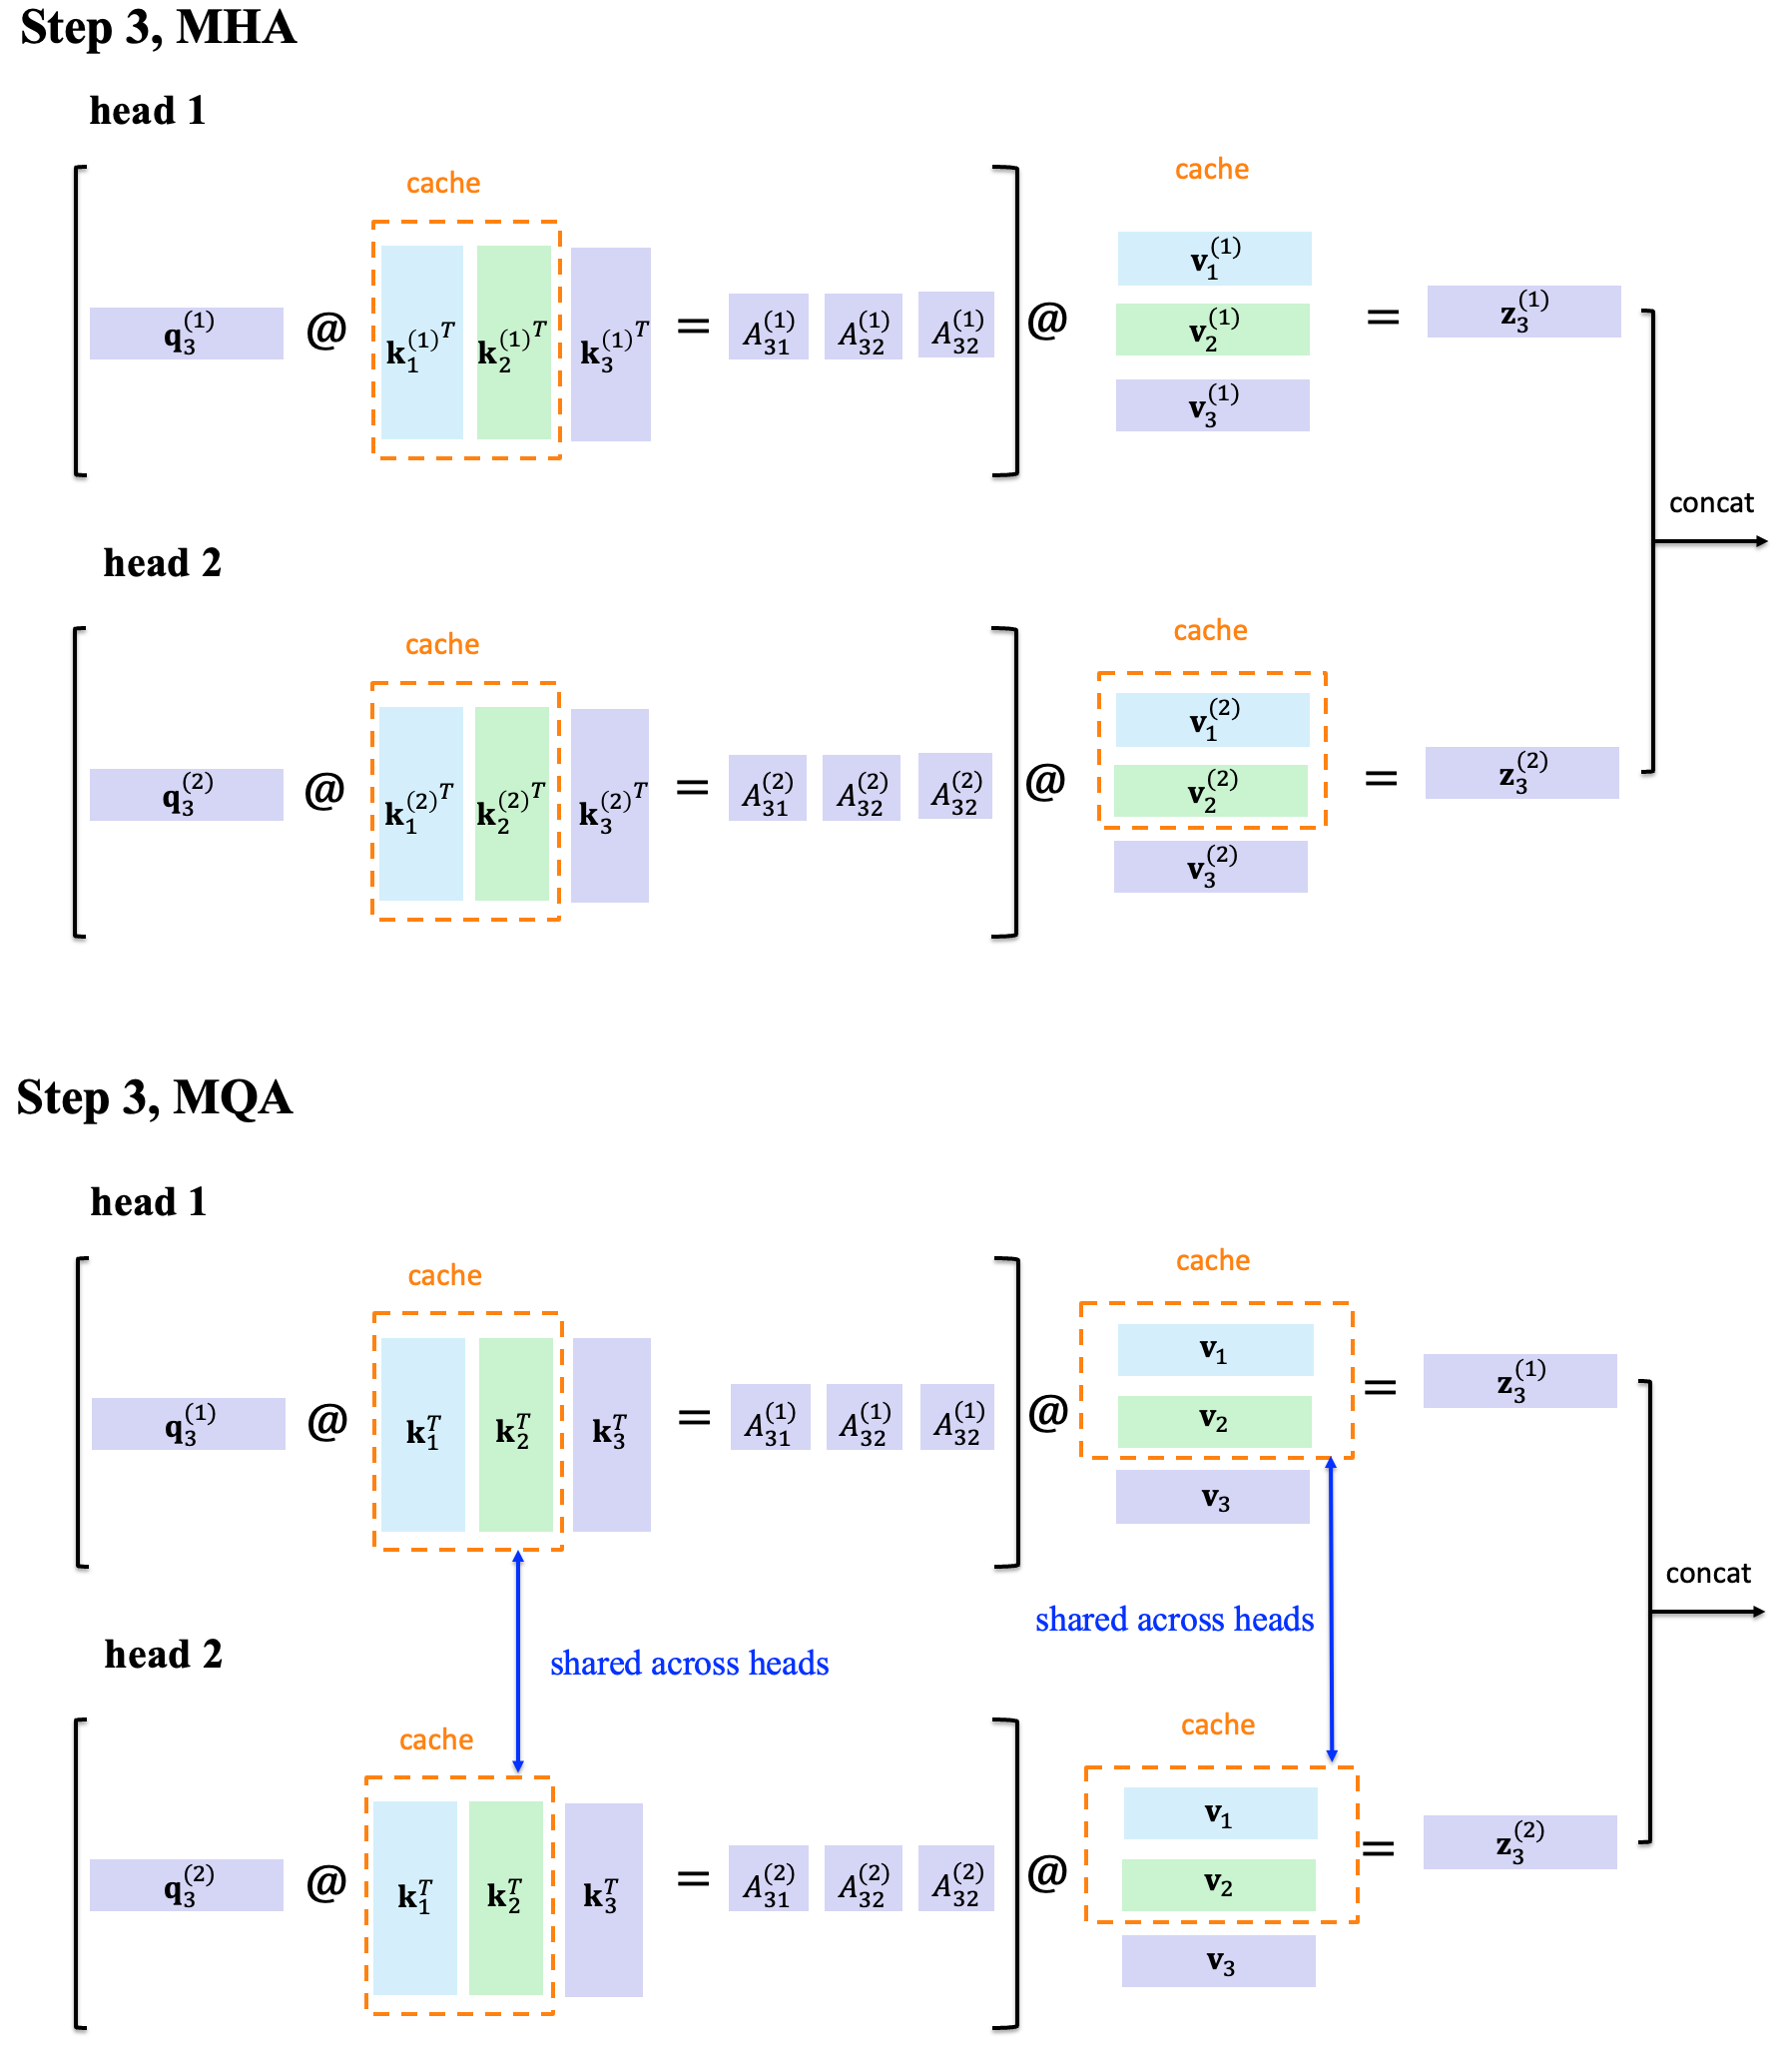
\includegraphics[scale=0.43]{imgs/MQA.png}
\end{figure}

\subsection{Grouped-Query Attention}
Sharing the key and value projection across all attention heads might be too brutal, in grouped-query attention, $\bW_K$ and $\bW_V$ are shared in grouped heads.
So basically different groups have different $\bK$ and $\bV$.

\begin{figure}[!h]
	\centering
	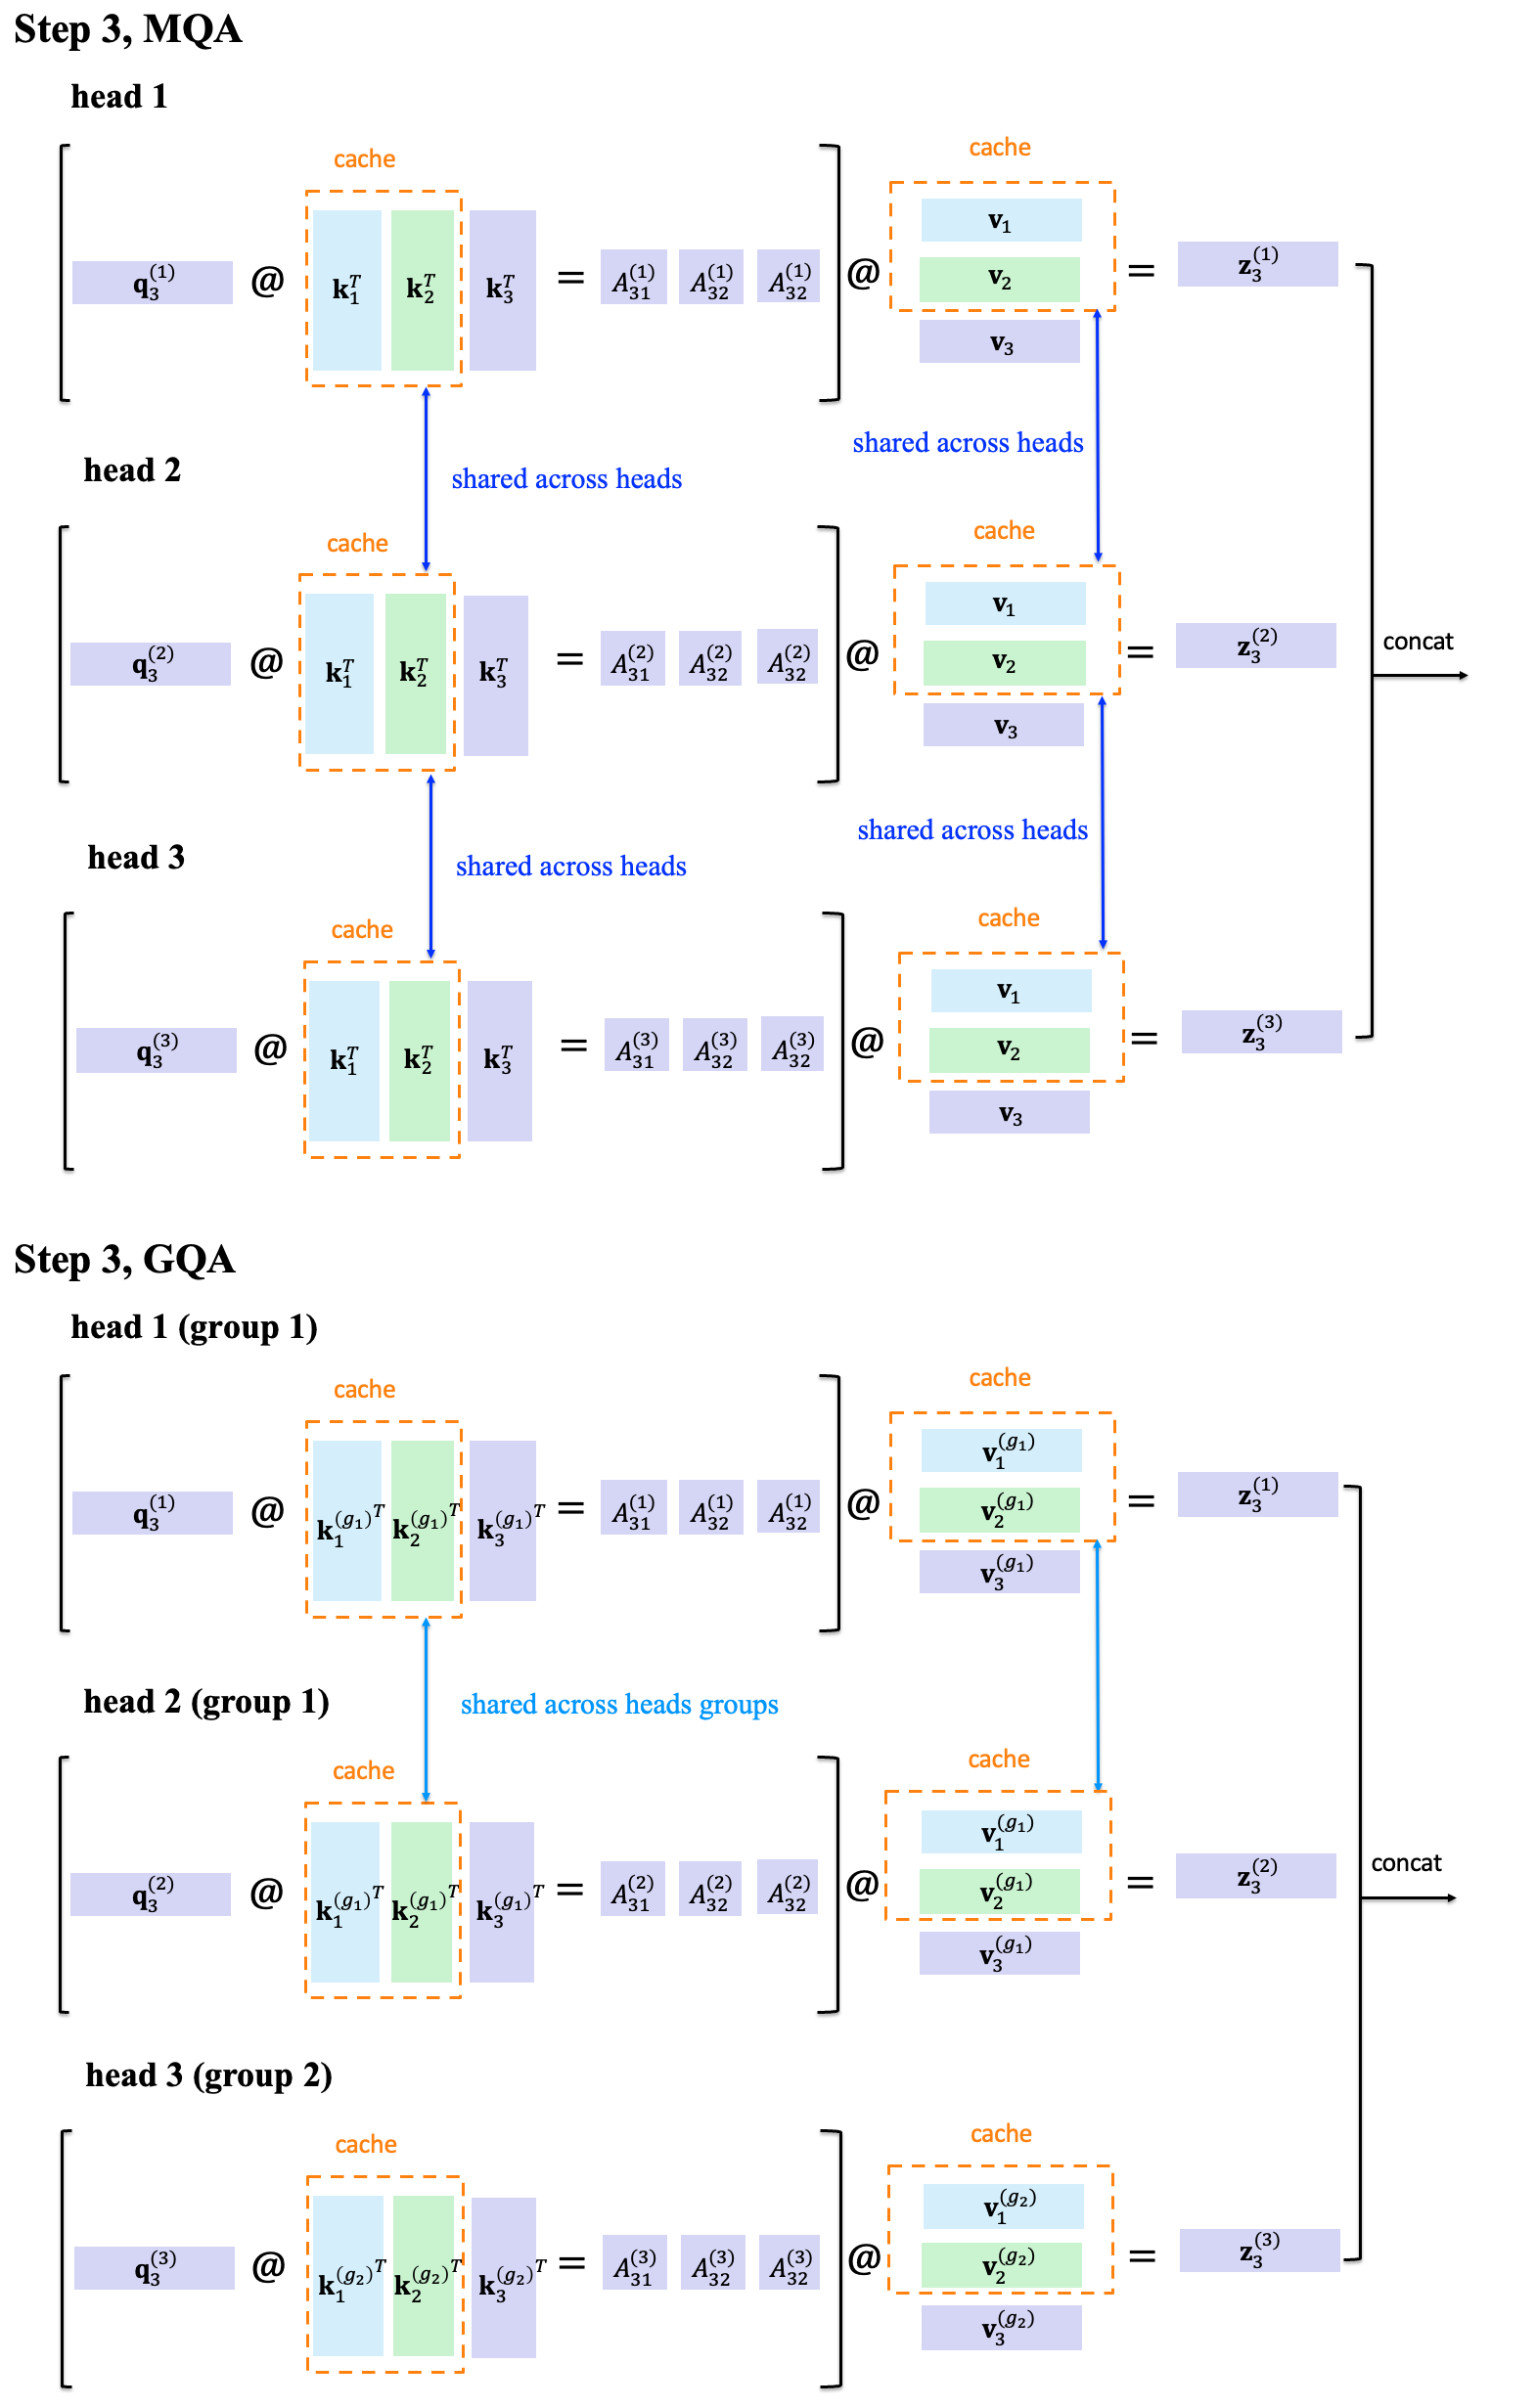
\includegraphics[scale=0.45]{imgs/GQA.png}
\end{figure}

\clearpage
\section{Positional Embedding}

\subsection{RoPE}


\paragraph{Once and for all vs add all the time}
In vanilla position embedding, it adds a vector at the beginning of the NN once and for all.
The positional encoding might get lost in deep networks.
If we look at the computation in transformer, the position only matters in the attention score computation.
So RoPE encode position into query and key vector in every attention layer instead.

\paragraph{Absolute position vs relative position}

Another thing RoPE did is encode the \textit{relative} position. 
The idea is, for a given word when computing its attention score, only the relative position between this word and other word should matter.
Specifically, if we add the position into the computation of query and key computation:
\[
\boldsymbol{q}_m \triangleq f_q(\boldsymbol{x}_m, m), \qquad  \boldsymbol{k}_n \triangleq f_k(\boldsymbol{x}_n, n)
\]

Then the attention score (which is an inner product) should only depends on the word embeddings $\boldsymbol{x}_m$, $\boldsymbol{x}_n$ and their relative position $m-n$:
\[
\boldsymbol{q}_m^{T} \boldsymbol{k}_n = \langle f_q(\boldsymbol{x}_m, m), f_k(\boldsymbol{x}_n, n) \rangle = g(\boldsymbol{x}_m, \boldsymbol{x}_n, m-n)
\]

One simple choice for $f_{\{q, k\}}(\boldsymbol{x}_m, m)$ is rotate them:
\[
f_{\{q, k\}}(\boldsymbol{x}_m, m) = \boldsymbol{R}(m) \boldsymbol{W}_{\{q, k\}} \boldsymbol{x}_m
\]
where $\boldsymbol{R}(m)$ is a rotation matrix whose angle depends on $m$.

Define $\widetilde{\boldsymbol{q}}_m =\boldsymbol{W}_q \boldsymbol{x}_m$ and $\widetilde{\boldsymbol{k}}_m =\boldsymbol{W}_k \boldsymbol{x}_m$, now we have
\[
(\boldsymbol{R}(m) \boldsymbol{W}_q \boldsymbol{x}_m)^{T} (\boldsymbol{R}(n) \boldsymbol{W}_k \boldsymbol{x}_n) = \widetilde{\boldsymbol{q}}_m^T \textcolor{mygreen}{\boldsymbol{R}(m)^T \boldsymbol{R}(n)} \widetilde{\boldsymbol{k}}_n = \widetilde{\boldsymbol{q}}_m^T \textcolor{mygreen}{\boldsymbol{R}(n-m)} \widetilde{\boldsymbol{k}}_n 
\]

Because rotation in higher dimension than 2D is not deterministic, it does a funky thing to split query vector in a bunch of 2D pairs, and then rotate them each.


\begin{figure}[!h]
	\centering
	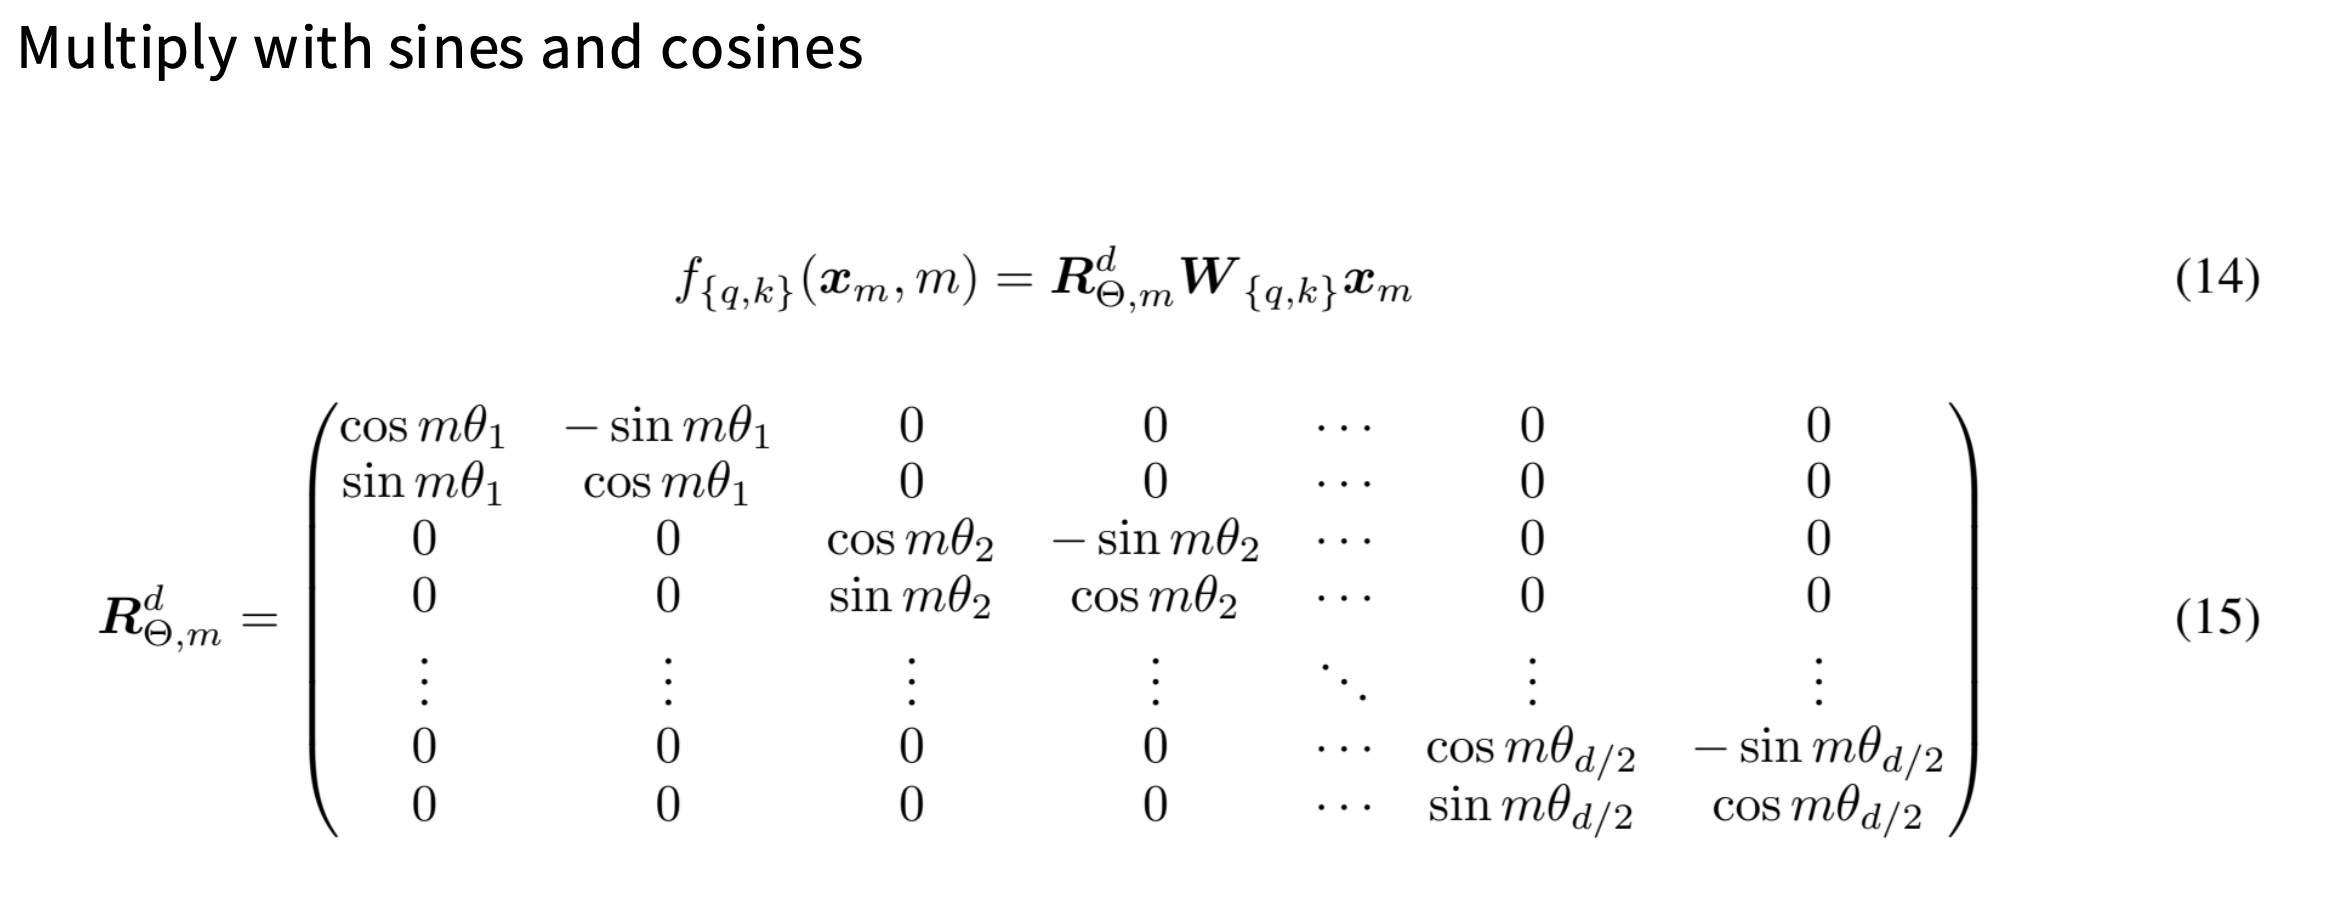
\includegraphics[scale=0.4]{imgs/rope.png}
\end{figure}


\begin{figure}[!h]
	\centering
	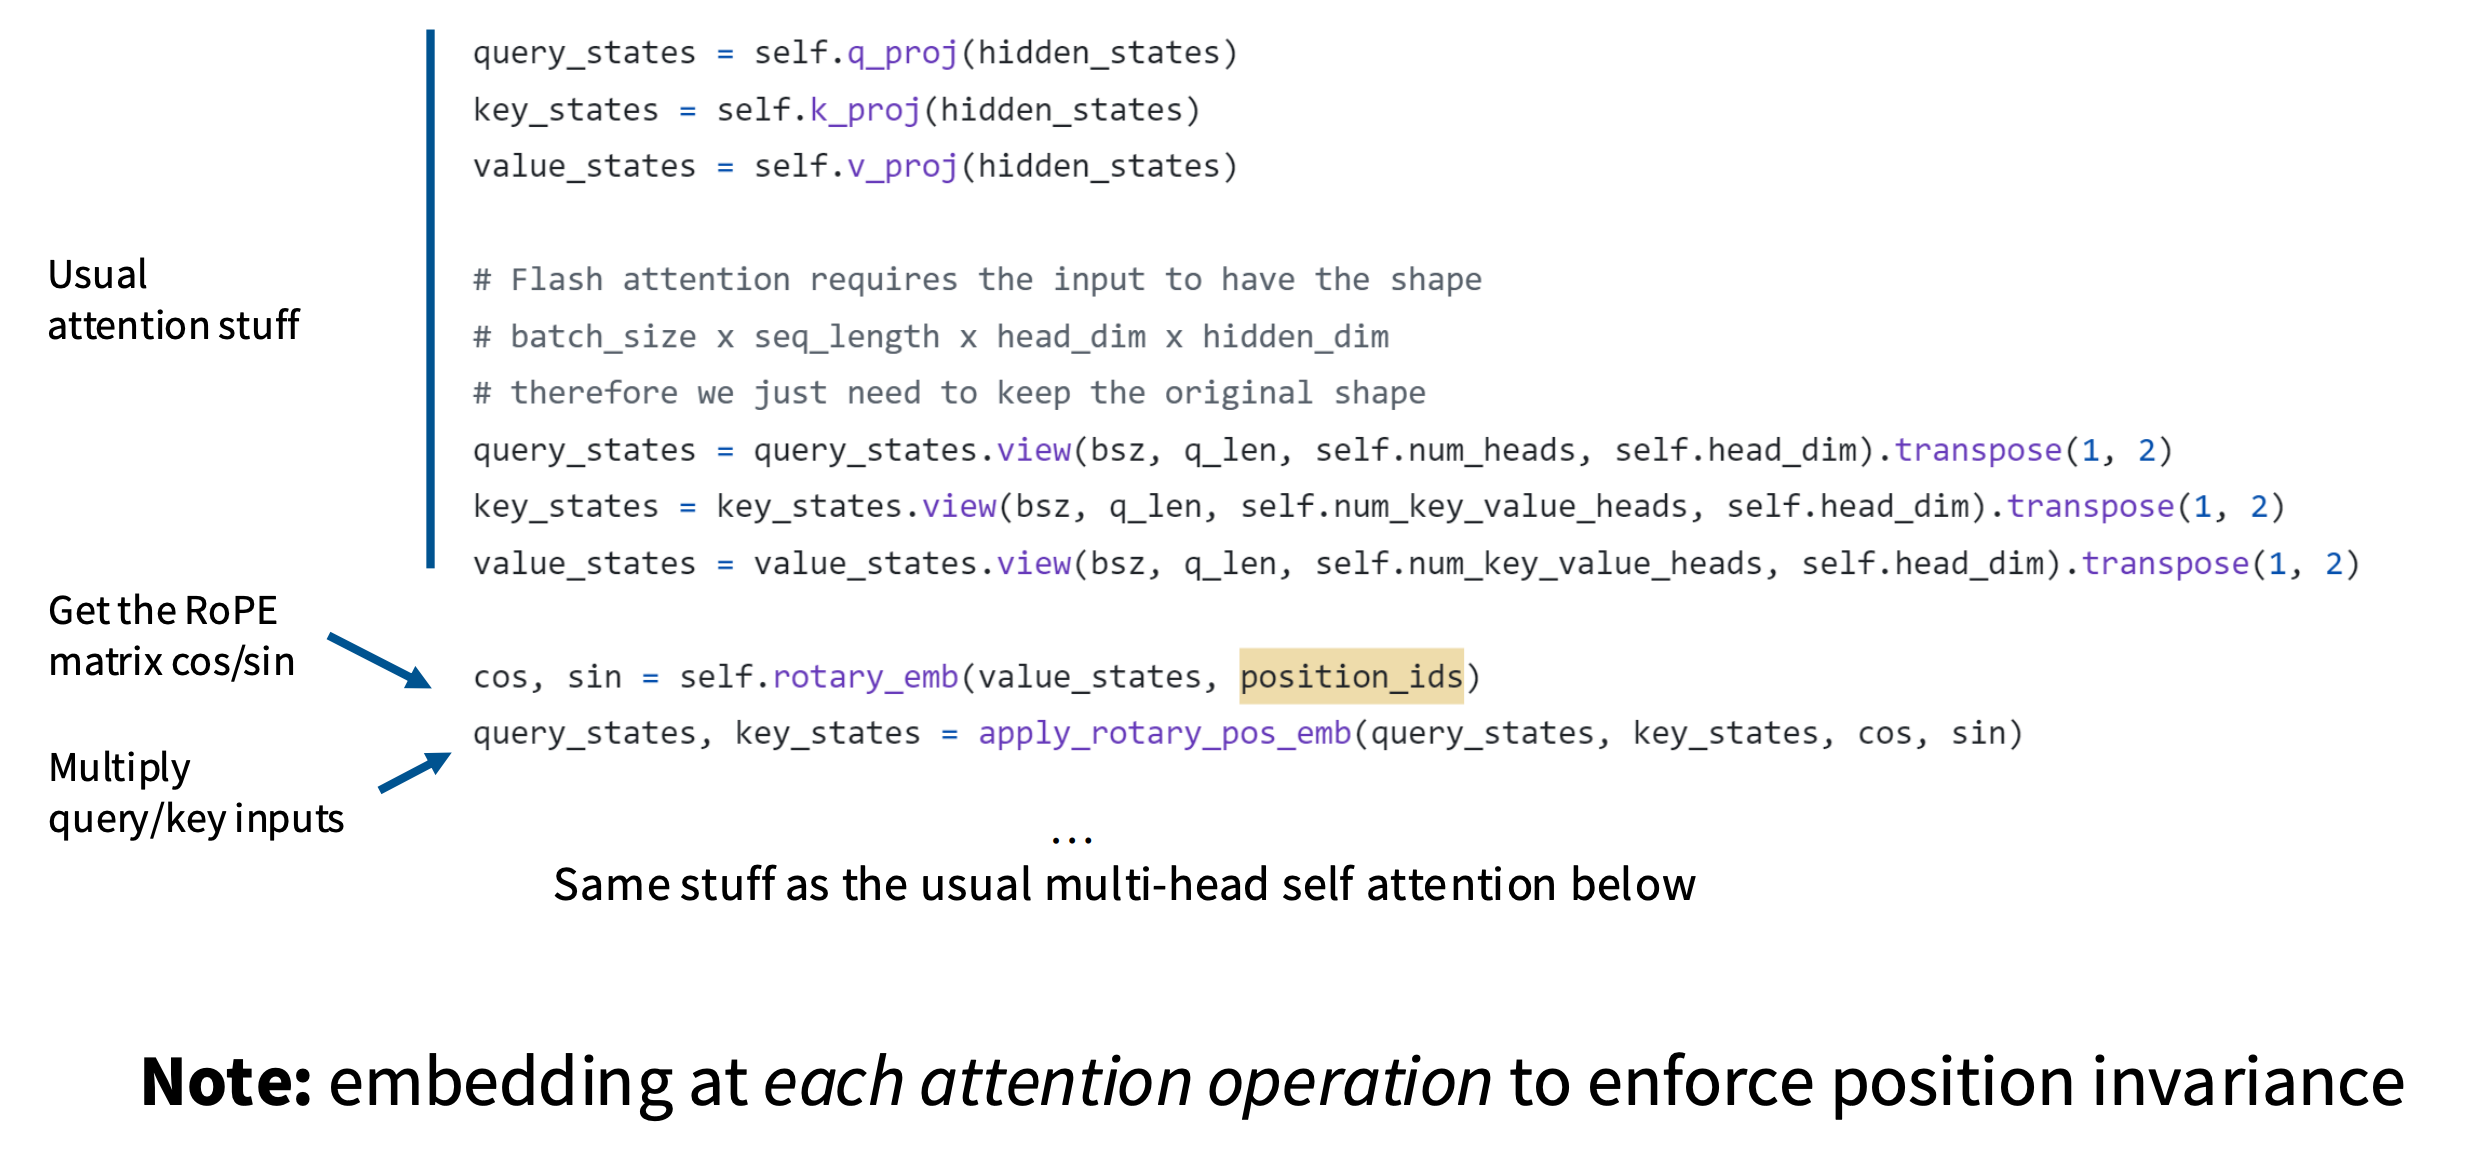
\includegraphics[scale=0.4]{imgs/rope-code.png}
\end{figure}

% print bibliography
\clearpage
\bibliography{bibliography} 

% Fill out appendix:
\newpage
\appendix

\end{document}
